% Theorie: Physikalische Grundlagen von Versuch/Messverfahren, Gleichungen ohne Herleitung knapp erklären
\section[Theorie]{Theorie \textnormal{\cite{photo}}}
\label{sec:theorie}

Bei Bestrahlung von Metalloberflächen mit Licht kann es zur Auslösung von Elektronen kommen. Dieses Phänomen wird als Photoeffekt
oder lichtelektrischer Effekt bezeichnet, zu seiner Beschreibung ist zunächst eine Einordnung der relevanten Eigenschaften von
elektromagnetischer Strahlung sinnvoll.

\subsection{Eigenschaften von Licht}

Die widerspruchsfreie Beschreibung aller experimentell nachgewiesenen Erscheinungen des Elektromagnetismus ist hochgradig nichttrivial
und erfordert komplexe mathematische Formulierungen. Ein solches Modell, das diesem Anspruch gerecht wird, ist in Form der Quantenelektrodynamik
gegeben. Als Grenzfälle enthält diese Quantenfeldtheorie wieder die klassischen Zusammenhänge, welche sonst nicht miteinander
vereinbar wären. Falls über eine große Anzahl von als Photonen bezeichneten Feldquanten gemittelt werden kann, ergibt sich die
Maxwellsche Welleninterpretation zur Beschreibung von Beugung und Interferenz. Bei Interaktionen von Licht mit Materie stellt
die Newtonsche Punktmechanik eine bessere Näherung dar und liefert Erklärungen für Beobachtungen wie den Compton-Effekt oder
die Paarbildung. Ansätze der zweiten Kategorie heißen auch Korpuskelinterpretionen.

\subsection{Lichtelektrischer Effekt}

Anordnungen zur Untersuchung des Photoeffekts wie in Abbildung~\ref{fig:prinzip} bestehen prinzipiell darin, eine Festkörperoberfläche
im Vakuum mit monochromatischem Licht zu bestrahlen. Neben der sogenannten Photokathode wird eine weitere Elektrode verbaut, welche
bezüglich dieser ein positives Potential besitzt. Letztere trägt auch die Bezeichnung der Auffängeranode. Es lassen sich einige
charakteristische Resulate solcher Versuche zusammenfassen:

\begin{enumerate}
	\item Der ausgelöste Elektronenstrom ist proportional zur Lichtintensität.
	\item Die kinetische Energie der Photoelektronen ist nur proportional zur Lichtfrequenz.
	\item Das Lösen von Elektronen tritt nur oberhalb einer bestimmten Grundfrequenz auf.
\end{enumerate}

\begin{figure}[H]
	\centering
	\hspace{4ex}
	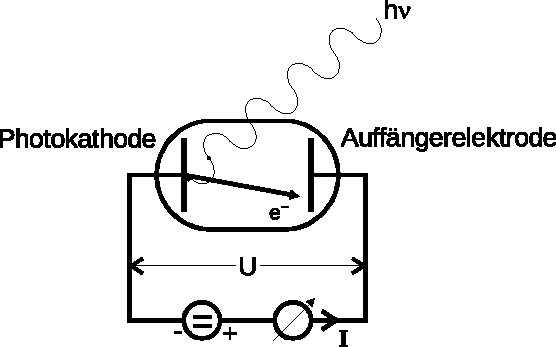
\includegraphics[width=0.5\linewidth]{content/grafik/prinzip.pdf}
	\caption{Prinzipielle Anordnung zur Untersuchung des Photoeffekts.}
	\label{fig:prinzip}
\end{figure}

Diese Beobachtungen lassen sich nicht mit einem Wellenmodell erklären. Ein solches würde die Elektronen als Oszillatoren betrachten, die
bei großer Schwingungsamplitude die elektrostatische Rückstellkraft überwinden können. Dann müsste jedoch deren kinetische
Energie mit der Intensität anwachsen. Ebenso gibt es in dieser Anschauung keine minimal notwendige Frequenz der Strahlung, da auch für
langwelliges Licht mit ausreichend hoher Intensität ein Auslösen möglich wäre. Zudem sollte durch Resonanzerscheinungen eine bevorzugte
Austrittsfrequenz existieren. 

In der Einsteinschen Korpuskulartheorie wird daher die Annahme der gleichmäßigen Energieverteilung über eine Wellenfront verworfen.
Stattdessen erfolgt der Transport von Strahlungsfeldenergie über konzentrierte Volumina mit praktisch verschwindender Ausdehnung 
im Raum. Diese Lichtquanten oder Photonen werden als identisch mit den Planckschen Energiequanten postuliert. Daraus folgen mehrere
relevante Schlüsse: Monochromatisches Licht der Frequenz~$\nu$ besteht gänzlich aus Photonen, die sich mit Lichtgeschwindigkeit~$c$
und Energie $h\nu$ geradlinig bewegen. Mit $h$ wird hier das Plancksche Wirkungsquantum bezeichnet. Überträgt ein Photon seine Energie
auf ein Elektron, teilt sich diese in Austrittsarbeit $A_k$ und kinetische Energie $E_k$ auf. Demnach gibt
\begin{align}
	h\nu = E_k + A_k
	\label{eqn:bilanz}
\end{align}
die Energiebilanz an und erklärt direkt die allgemeine Proportionalität von kinetischer Energie der Photoelektronen zur Frequenz sowie
für $h\nu < A_k$ das Auftreten einer unteren Grenze. Weiter folgt aus der Theorie, dass die Intensität der Strahlung proportional
zur Anzahl der Photonen pro Fläche und Zeit ist. Da ein Photon jeweils nur maximal ein Elektron aus der Metalloberfläche auslösen kann,
wächst der Strom also wie beobachtet mit der Intensität an.
\\[5em]
\subsection{Grundlagen der Apparatur}

Der eigentliche lichtelektrische Effekt findet in einem dazu evakuierten Glaskolben, der sogenannten Photozelle statt. Die Kathode besteht
dabei aus einer auf der Innenseite zur Bestrahlung aufgedampften Metallschicht. Wie in Abbildung~\ref{fig:photozelle} ist diese von
einer kreisförmigen Ringanode umgeben.

\begin{figure}[H]
	\centering
	\hspace{12.5ex}
	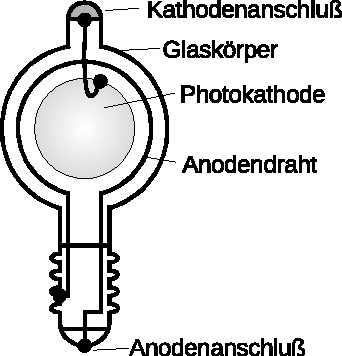
\includegraphics[width=0.3\linewidth]{content/grafik/photozelle.pdf}
	\caption{Schematische Darstellung der verwendeten Photozelle.}
	\label{fig:photozelle}
\end{figure}

Zur Erzeugung von monochromatischer Strahlung verschiedener Frequenzen dient eine Spektrallampe. Das Licht wird durch die
Kondensorlinse gebündelt, die Abbildungslinse wirft ein Bild der Spaltblende auf den Eintrittsspalt. Ein Geradsichtprisma
sorgt für die notwendige räumliche Trennung der für den jeweiligen Übergang spezifisch emittierten Spektrallinien, ohne dass
die optische Achse verschoben wird. Je nach eingestelltem Winkel des Schwenkarms trifft so eine andere Lichtfarbe auf die Photokathode.
Die hier beschriebene Funktionsweise kann in Abbildung~\ref{fig:optik} nachvollzogen werden.

\begin{figure}[H]
	\centering
	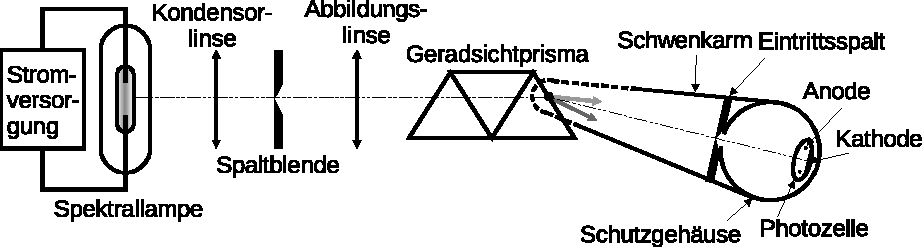
\includegraphics[width=0.8\linewidth]{content/grafik/optik.pdf}
	\caption{Optischer Teil des Versuchsaufbaus.}
	\label{fig:optik}
\end{figure}
\vspace{-1em}
Der Aufbau ist so zu justieren, dass in der Ebene der Spaltblende ein Bild entsprechend dessen Breite entsteht. Mit den Parametern
Brennweite~$f$, Gegenstandsweite~$g$, Bildweite~$b$, Gegenstandsgröße~$G$ und Bildgröße~$B$ können die Beziehungen für dünne Linsen
\begin{align}
	f = \pfrac{bg}{\hspace{0.1ex}b + g\hspace{0.1ex}} && \pfrac{G}{B\hspace{0.2ex}} = \pfrac{g}{b\hspace{0.2ex}}
	\label{eqn:linse}
\end{align}
genutzt werden, um die Einstellung rechnerisch vorzubereiten.

\begin{figure}[H]
	\centering
	\hspace{6ex}
	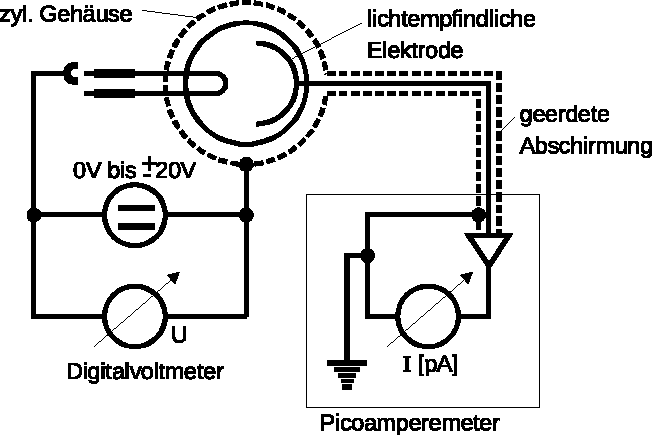
\includegraphics[width=0.6\linewidth]{content/grafik/schaltbild.pdf}
	\caption{Elektrisches Schaltbild der Messapparatur.}
	\label{fig:schaltbild}
\end{figure}

Zur Messung der Energien wird mit der Schaltung in Abbildung~\ref{fig:schaltbild} die Gegenfeldmethode umgesetzt. Zur Abschirmung möglicher
Störfelder werden für die Zuleitungen geerdete Koaxialkabel verwendet. Mit $e_0$ und $m_0$ sind die Naturkonstanten Elementarladung
und Ruhemasse des Elektrons bezeichnet. Es erreichen nur solche Ladungsträger die Anode, deren kinetische Energie größer als die Feldenergie
ist. Bei
\begin{align}
	e_0 U_{\hspace{-0.2ex}g} = \pfrac{1}{2} m_0 v_0^2
	\label{eqn:null}
\end{align}
verschwindet also der Photostrom, entsprechend lässt sich aus der Gegenspannung $U_{\hspace{-0.2ex}g}$ die Energie der schnellsten Elektronen
mit maximaler Geschwindigkeit $v_0$ bestimmen. Wird dies in die vorherige Beziehung der Frequenzabhängigkeit eingesetzt, ergibt sich
\begin{align}
	h\nu = e_0 U_{\hspace{-0.2ex}g} + A_k
	\label{eqn:maximal}
\end{align}
als Energiebilanz. Die Messung wird weiter erschwert, da der Strom bei $U_{\hspace{-0.2ex}g}$ nicht diskret auf Null abfällt, sondern bereits
zuvor wie in Abbildung~\ref{fig:kurve} deutlich sinkt. 

\begin{figure}[H]
	\centering
	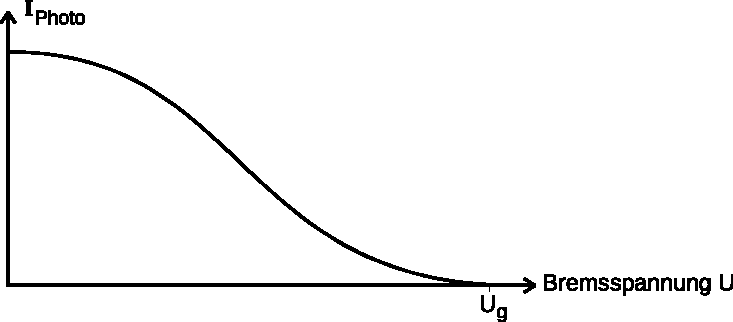
\includegraphics[width=0.7\linewidth]{content/grafik/kurve.pdf}
	\caption{Photostrom in Abhängigkeit von der Bremsspannung.}
	\label{fig:kurve}
\end{figure}

Begründen lässt sich dieses Phänomen damit, dass die Energieverteilung der Elektronen im Festkörper bereits einer kontinuierlichen
Fermi-Dirac-Statistik folgt. Diese besagt, dass sowohl für Leitungselektronen als auch Valenzelektronen alle kinetischen Energien zwischen
Null und der Fermi-Energie $\zeta$ vorkommen. Durch thermische Effekte treten zudem noch Ausreißer mit weit höheren Energien auf. Für die
vorliegende Apparatur kann zwischen Photostrom $I$ und Bremsspannung $U$ mit
\begin{align}
	I \sim U^2
	\label{eqn:parabel}
\end{align}
ein parabolischer Zusammenhang angenommen werden.

\begin{figure}[H]
	\centering
	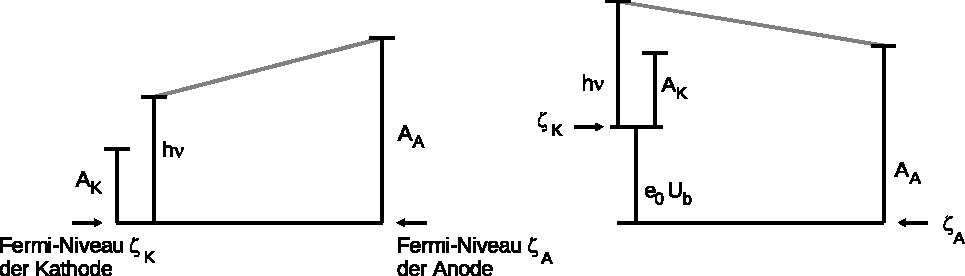
\includegraphics[width=0.9\linewidth]{content/grafik/potential.pdf}
	\caption{Potentialverhältnisse zwischen Anode und Kathode.}
	\label{fig:potential}
\end{figure}
\vspace{-2ex}
Ein zusätzliches Problem tritt auf, falls zwischen den Austrittsarbeiten der Kathode $A_k$ und der Anode $A_a$ ein Verhältnis $A_k \ll A_a$
herrscht. Dann gibt es für $A_k < h\nu < A_a$ kinetische Energien, bei denen zwar Elektronen gelöst werden, diese aber nicht die Anode erreichen.
Ein solcher Fall ist links in Abbildung~\ref{fig:potential} dargestellt. Um trotzdem geringere Frequenzen untersuchen zu können, wird eine
Beschleunigungsspannung $U_b$ mit
\begin{align}
	h\nu + e_0 U_b \geq A_a
	\label{eqn:potential}
\end{align}
angelegt, sodass das Potential eine Gestalt wie rechts in Abbildung~\ref{fig:potential} annimmt. Zuletzt ist noch zu beachten, dass für
große Bremsspannungen ein negativer Strom auftreten kann, welcher den eintreffenden Strom überlagert und die Messwerte verfälscht.

